\section{Experimental Details}

Equilibrium molecular dynamics simulations of a symmetric binary--mixture of partially miscible fluids were used to measure the stresses acting on the fluid at two different temperatures.
The Marangoni force was then inferred using Equation \ref{FinDiff}.
Where possible, this force was applied as a body force in a simulation at an intermediate temperature to generate a Marangoni flow profile.

Two key systems were studied, a symmetric binary–mixture under three--dimensional periodic boundary conditions, and a binary--mixture periodic in the $(x,y)$ plane but confined between two walls in the $z$--dimension, as shown in Figure \ref{SetUp}.
All molecular dynamics simulations were executed using the LAMMPS (Large Atomic and Molecular Massively Parallel Simulator) package.\cite{LAMMPS}  
\begin{figure}[h]
	\begin{subfigure}{.5\linewidth}
		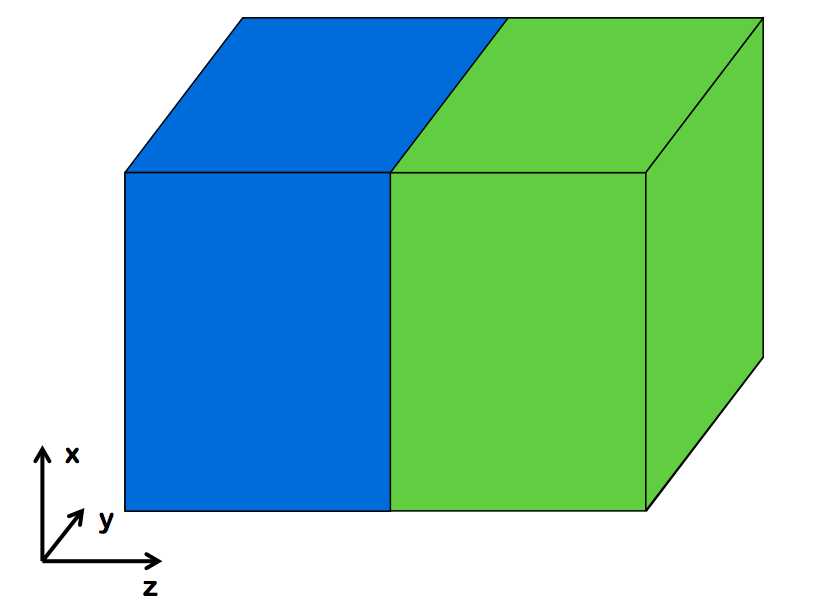
\includegraphics[scale=0.25]{AABB.png}
		\caption{Binary--mixture periodic in all dimensions}
		\label{AABB}
	\end{subfigure}
	\begin{subfigure}{.5\linewidth}
		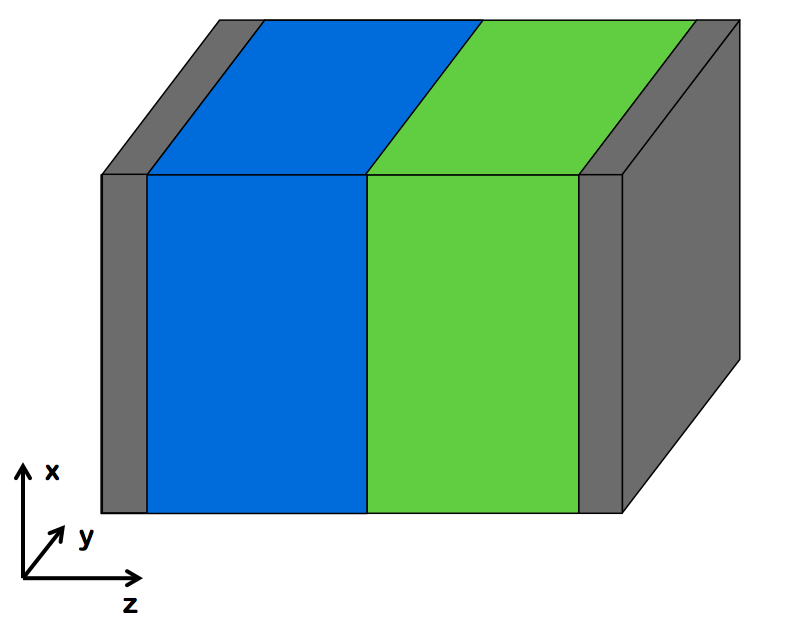
\includegraphics[scale=0.25]{AABB_piston.png}
		\caption{Binary--mixture confined by planar walls} 
		\label{AABB_piston}
	\end{subfigure}
	\caption{Both the systems studied incorporated a partially miscible binary--mixture of Fluid A (blue) and Fluid B (green).
For the mixture periodic in all dimensions, the pressure is regulated using a Nos\'{e}--Hoover barostat.
In the confined fluid, the walls are used to create a piston and an external force equal to $P_{\mathrm{ext}} \times A_{\mathrm{wall}}$ is applied.
}
	\label{SetUp}
\end{figure}

\subsection{Interaction model}\label{InteractionModel}
The fluids were modelled using spherical particles and their interaction was tuned to a pair--wise truncated Lennard--Jones potential:
\begin{equation}
V \left( \mathbf{r}^{\mathrm{N}} \right) = \frac{1}{2} \sum_{i\neq j} \phi \left( r_{ij} \right)
\end{equation}
where
\begin{align}
\label{LJ}
\phi \left( r_{ij} \right) &= 4 \epsilon_{ij} \left( \left( \frac{\sigma_{ij}}{r_{ij}}\right)^{12} - \left( \frac{\sigma_{ij}}{r_{ij}}\right)^{6} \right)\ \mathrm{for}\ r \leq r_{c}\\
\phi \left( r_{ij} \right) &= 0\ \mathrm{for}\ r > r_{c}.
\end{align}
This potential includes an attractive $r_{ij}^{-6}$ term accounting for long--range dispersion forces and a short--range $r_{ij}^{-12}$ repulsive term corresponding to the Pauli repulsion between particles.
The length--scale of the potential is given by $\sigma_{ij}$ (set as equal for all $i$ and $j$) while $\epsilon_{ij}$ determines the strength of the interaction. 

The miscibility of the two fluids (A and B) was controlled using the relative values of the interaction parameter.
The values chosen were:
\begin{align}
\epsilon_{A,A} &= \epsilon_{B,B} = 1.0,\\
\epsilon_{A,B} &= 0.55,
\end{align}
in agreement with previous studies on Lennard--Jones binary--mixtures.\cite{MorenzoRazo,Blas,HolgerBoppHampe}
The cutoff for the potential was $r_{c} = 4\ \sigma$.

\subsection{Reduced units}\label{ReducedUnits}
Physical quantities including distances and energies are expressed in terms of reduced units.
For a Lennard--Jones system, the basic units are $\sigma$ for length, $\epsilon$ for energy and $m$ for mass, from which all other units may be derived.\cite{FrenkelSmit}
Physical quantities become dimensionless when expressed in terms of these units, for example $r^{*} \equiv r / \sigma$.
Scaled coordinates expressed relative to the simulation box size are also used, for example $z' = z^{*} / L_{z^{*}}$ where $L_{z^{*}}$ is the dimension of the box in the z--direction.
These are useful if the box--dimensions vary, such as when a barostat acts on the system.

\subsection{Thermostats}\label{Thermostats}
In molecular dynamics simulations, the temperature is controlled using thermostats, which simulate the coupling of the system to an external heat bath.

Thermostats work by applying a stochastic frictional force to particles, either by adding a random force to momenta (Langevin)\cite{Langevin} or reassigning the velocity of randomly chosen particles to that obtained from the Maxwell distribution (Andersen)\cite{AndersonTherm}.
The Nos\'{e}--Hoover thermostat was used throughout this study.
This introduces a fictitious frictional force into the equations of motion, adjusting the particle velocities until the temperature is equal to the desired value.\cite{NoseHoover1, NoseHoover2, NoseHoover3}
The equations of motion in three--dimensions become:
\begin{align}
m_{i}\frac{\mathrm{d}^{2}\mathbf{r}_{}}{\mathrm{d} t ^{2}} =& \mathbf{f}_{i} - \zeta m_{i} \mathbf{v}_{i}\\
\frac{\mathrm{d} \zeta (t)}{\mathrm{d} t} =& \frac{1}{Q}\left[ \sum_{i=1}^{N} m_{i} \frac{\mathbf{v}^{2}_{i}}{2} - \frac{3N+1}{2}k_{\mathrm{B}}T\right].
\end{align}
The result is a system where the energy fluctuates but the combined energy of the system and heat bath remains constant, maintaining a canonical ensemble.

\subsection{Barostats}\label{Barostats}
The bulk pressure of the fluid must also be held constant.
A piston provides the simplest method; the fluid is confined between two solid walls and a force equal to $P_{ext} \times A_{wall}$ is applied.
This was used for studying the binary--mixture confined between two walls.
Under a temperature gradient, a thermocapillary effect also occurs at the liquid--solid surface.
The interface must be sufficiently far from the walls such that this can be ignored.

Alternatively a Nos\'{e}--Hoover barostat regulates the pressure by adjusting the simulation box dimensions and altering the equations of motion accordingly. \cite{NoseHoover1, NoseHoover2, NoseHoover3}
When studying surface effects, the box size must only be changed in the direction perpendicular to the interface.
A change parallel to the interface adjusts its area and creates an error in the thermodynamic pressure,
\begin{equation}
P = - \left( \frac{\partial F}{\partial V} \right)_{T} + \gamma \left( \frac{\partial A}{\partial V} \right)_{T}.
\end{equation}

\subsection{Preparing the system}\label{SystemPrep}
The fluid was prepared from a face--centred cubic lattice with a spacing of $1.64414\ \sigma$ and a simulation box size of $L_{x^{*}}=13.1531$, $L_{y^{*}}=13.1531$ and $L_{z^{*}}=32.8828$.
This lattice was melted over $2\times 10^{6}$ timesteps of length $0.001\ \tau$ to generate a fluid state.
The pressure was $P^{*} = 0.1$ and the temperatures used were $T^{*} = 0.8$ and $T^{*} = 0.9$, ensuring the system occupied the liquid region of the Lennard--Jones phase space.\cite{Smit}
Solid walls were constructed with a harmonically bonded lattice using a spring constant of $K^{*} = 2500$ and an equilibrium bond length of $r^{*}_{0}=1.163$.

\subsection{Calculating the stress tensor}\label{CalcStress}
The virial stress tensor was calculated using an in--built function within the LAMMPS package, which returns the stress tensor for each atom.
However, LAMMPS does not have a method for calculating the Irving--Kirkwood stress tensor.
Instead this was calculated by saving the particle positions on a given timestep to a file.
The stress tensor was then computed using a programme written by R. Ganti and adapted for the specific systems studied.
Since the virial method is implemented in parallel whilst the Irving--Kirkwood method is not, computing the Irving--Kirkwood stress incurred approximately a 4-fold increase in computational time.

\subsection{Computing averages}\label{ComputeAve}
Usually time--averages of physical observables are calculated in molecular dynamics simulations. 
In this study, the observables are the number density, stress tensor and particle velocities.
Their values were measured on every timestep and spatially averaged into $400$ planar slabs across the z--dimension of the box.
These spatial averages were then time--averaged over the full simulation.

Under the ergodic hypothesis, time--averages can be equated to ensemble averages for an infinitely long simulation time.\cite{Bopp2008}
Practically, however, these averages are evaluated over a finite time period, and have a statistical error.
The method of block--averaging, developed by Flybjerg and Peterson, provides an efficient technique for computing this error.\cite{Flyvbjerg1989}
They show that the variance of an observable, $A$, can be estimated by
\begin{equation}
\mathrm{var}(A) \geq \left< \frac{C_{0}}{n-1} \right>,
\end{equation}
where $C_{0}$ is the value of the time-correlation function for the block--transformed data at $t=0$ given by
\begin{equation}
C_{0} \equiv \frac{1}{n} \sum_{k=1}^{n} \left( A_{k} - \bar{A} \right) \left(A_{k} - \bar{A} \right).
\end{equation}
A lower bound for the variance can be calculated by finding the block length where this estimate plateaus.
Furthermore, the error in the variance can be estimated as 
\begin{equation}
\sqrt{\frac{2}{n-1} \times \frac{C_{0}}{n-1}}.
\end{equation}

\begin{figure*}[h]
\hspace{-3em}
	\begin{subfigure}{.5\linewidth}
                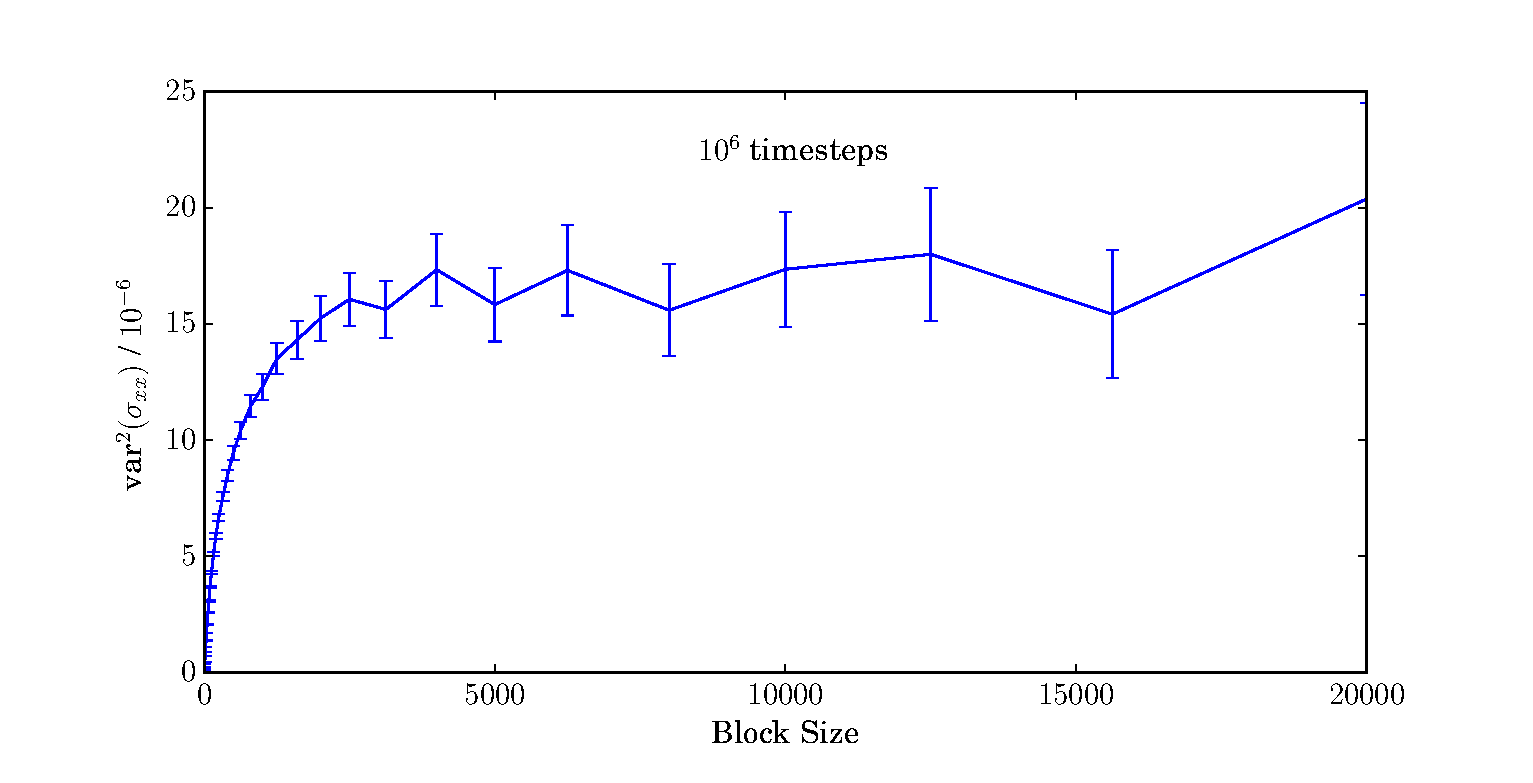
\includegraphics[scale=0.6]{block_average_1e6.eps}
                \caption{Simulation time = $1000\ \tau$}
        \end{subfigure}
\hspace{2em}
        \begin{subfigure}{.5\linewidth}
                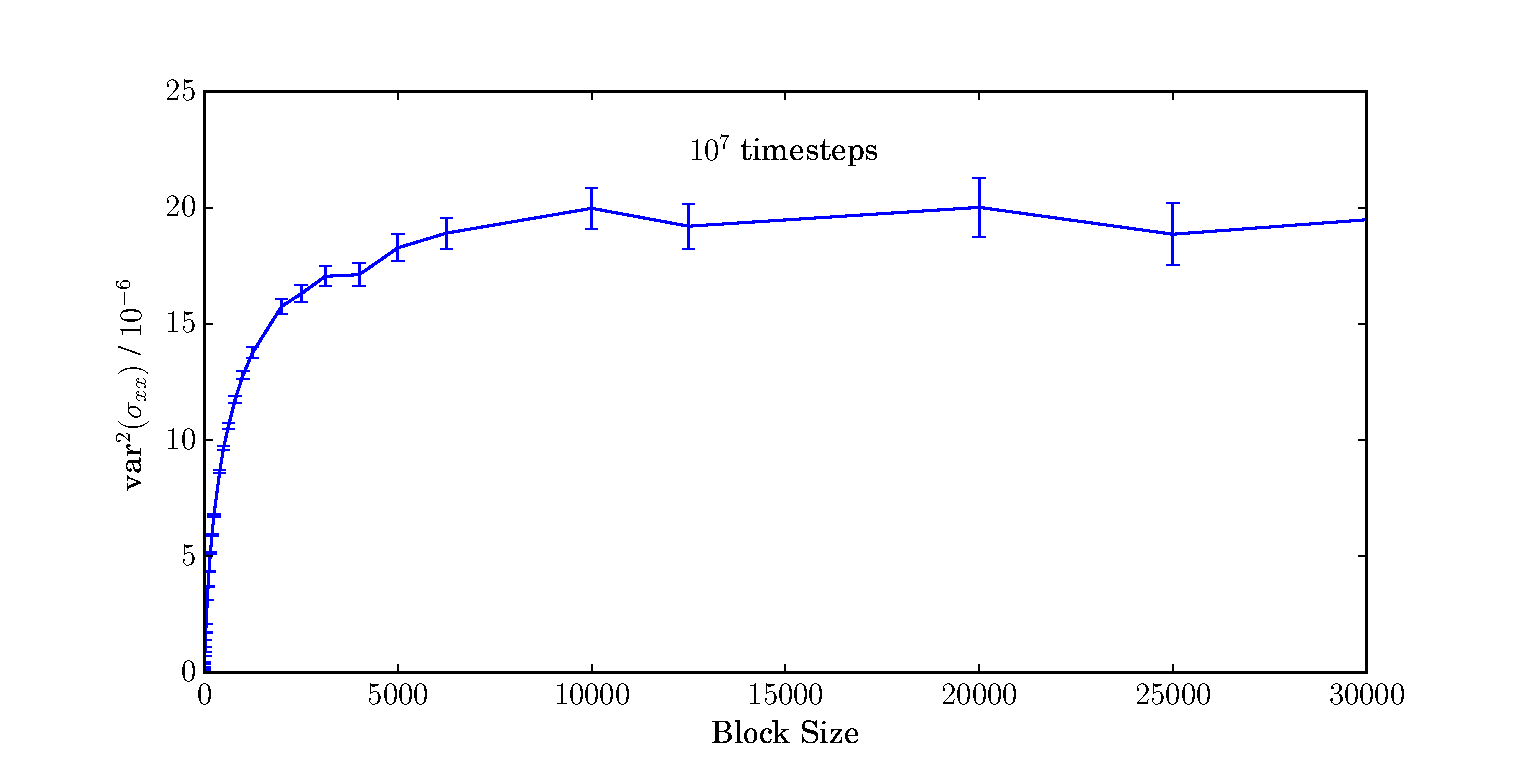
\includegraphics[scale=0.6]{block_average_10e6.eps}
                \caption{Simulation time = $10000\ \tau$}
	\end{subfigure}
	\caption{The blocking analysis for a system identical to those studied is compared for simulation times of $1000\ \tau$ and $10000\ \tau$.
Plateaus in the estimate of the variance begin at block lengths of approximately $5\ \tau$ and $10\ \tau$ respectively.
The error in the variance does not become significant until much larger block lengths.
Throughout the subsequent simulations, a block size of $10\ \tau$ was used.
This ensured decorrelation of the data and produced a reliable estimate of the statistical error.
}
\label{blocking}
\end{figure*}

A blocking--analysis for a binary--mixture identical to those used throughout this study was executed over a simulation time of $1,000\ \tau$ and $10,000\ \tau$, as shown in Figure \ref{blocking}.
The plateau begins at a block length of $10\ \tau$ for the long simulation and $5\ \tau$ for the shorter run, with little increase in the error of the variance until a much larger block size is reached.
Consequently, a block length of $10\ \tau$ was used to estimate the error of all time--averages calculated in the subsequent simulations.
\FloatBarrier

\subsection{Modelling surfactant molecules}\label{ModellingSurfactants}
\begin{figure*}[h]
\centering
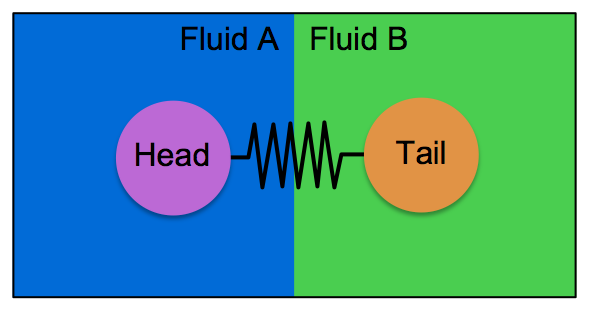
\includegraphics[scale=0.4]{surfactant.png}
\caption{Surfactant molecules were represented by a pair of spherical Lennard--Jones particles connected by a harmonic bond. 
The head particle has a stronger interaction with Fluid A ($\epsilon_{H, A} = 1.33$ and $\epsilon_{H, B} = 0.17$) whilst the tail has a stronger interaction with Fluid B ($\epsilon_{T, A} = 0.17$ and $\epsilon_{T, B} = 1.33$).
This imitates the behaviour of non--ionic surfactant molecules.
 }
\label{surfactant}
\end{figure*}
To investigate the effects of surfactants on Marangoni flows, surfactant molecules were modelled as a pair of Lennard--Jones particles connected by a harmonic bond with spring constant $K^{*} = 25$ and equilibrium bond length $r^{*}_{0}=1.63$.
Inspired by Howes and Radke's study on non--ionic surfactants,\cite{HowesSurfactant} the `head' particle has a stronger interaction with Fluid A particles, ($\epsilon_{H, A} = 1.33$ and $\epsilon_{H, B} = 0.17$) whilst the `tail' particle has a stronger interaction with Fluid B particles ($\epsilon_{T, A} = 0.17$ and $\epsilon_{T, B} = 1.33$).
The `head' and `tail' groups interact with each other with strength $\epsilon_{H, T} = 1.00$.
\FloatBarrier

\subsection{Software details}\label{SoftwareDetails}
All molecular dynamics simulations were run using the LAMMPS package.\cite{LAMMPS}
Additional processing was executed using NumPy.\cite{NumPy}
Graphical figures were plotted using matplotlib.\cite{MatPlotLib}

